\chapter{Search for X17}
\begin{refsection}
\label{ch:X17}
{\itshape After the recent publications from the ATOMKI collaboration, the so-called X17 anomaly peaked the interest of the community. The flexibility of the MEG II apparatus allows for a variety of exotic searches and the collaboration is deemed of interest in searching for this anomaly in an uncorrelated way.
The chapter starts with a recap of the previous searches and then moves to the description of this search in MEG: setup used; simulations developed; data acquisition and data analysis.}

\section{ATOMKI and the X17 `anomaly'}
    The story of the Hungarian group and their result
\section{MEG II setup}
    \subsection{Magnetic \textbf{B} field}
    \subsection{Target}
        \paragraph{Tube and insertion}
        \paragraph{Vacuum and mechanical structure}
        \paragraph{Lithium target}
    \subsection{MC simulations}
\section{Data acquisition}
    \subsection{Beam tuning}
        The beam tuning was performed by substituting the end-cap of the proton beam line with a transparent cap with a AAA crystal. 
        The proton beam produces visible photons hitting the crystal so the beam position can be observed.
        Normally this operation would be done while the upstream side of COBRA is not closed, allowing the installation of a webcam that gives instant feedback on the beam position.
        This was not the case so we were forced to use the camera installed inside COBRA for MEG II target monitoring.
        This camera has some settings for \textit{gain} and \textit{aperture} but is controlled using a script in \textit{ssh} and to view the picture first is necessary to move them locally, making the whole procedure somewhat cumbersome.
        Key aspects of the beam to be tuned were: 
        \begin{outline}
            \1 Energy: This parameter is controlled by the \textit{Terminal Voltage} of the CW.
            \1 Focus: This parameter is controlled by the \textit{Extraction Voltage} of the CW. Fig.~\ref{} shows how the beam spot changes as a function of this parameter. 
            \1 Position: This parameter is controlled by the three dipoles of the CW beamline. The change of the position for different values of the dipoles at \SI{500}{keV} is shown in Fig.~\ref{fig:position_500keV}.
        \end{outline}

        \begin{figure}
            \centering
            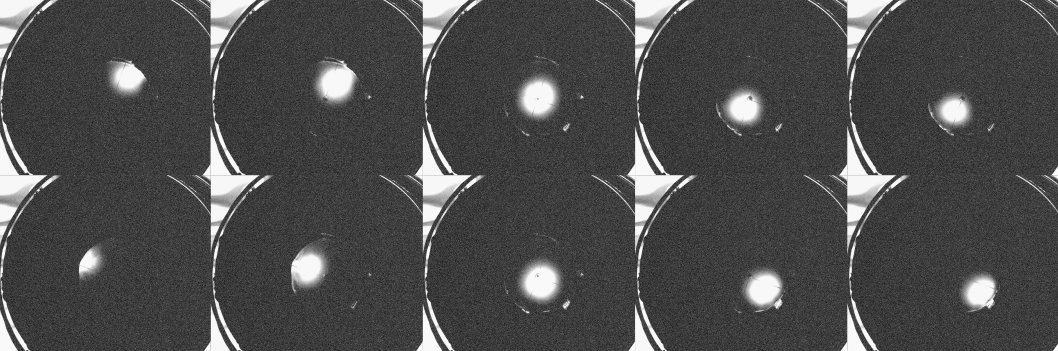
\includegraphics[width = \textwidth]{Figures/MEG/X17/beamtuning/psotion_500keV.png}
            \caption{Position of the proton beam at \SI{500}{keV} when changing the current in the dipoles (the vertical dipole V and only one of the two horizontal dipoles H). In the first row, H(??) is changing and the beam moves diagonally. In the second row, V(??) moves the beam on the perpendicular diagonal.}
            \label{fig:position_500keV}
        \end{figure}
        \begin{figure}
            \centering
            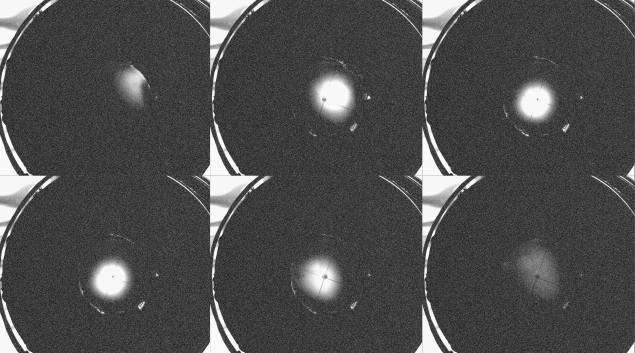
\includegraphics[width = \textwidth]{Figures/MEG/X17/beamtuning/focus_500keV.png}
            \caption{Focus of the proton beam at \SI{500}{keV} when changing the \textit{extraction voltage} of the CW: values in the range $6\divisionsymbol15$ keV. Is clearly visible for extreme values the beam barely reaches the crystal.}
            \label{fig:ocus_500keV}
        \end{figure}
        After a careful scan of the three parameters, working points at different energies were chosen: the most relevant are the ones for \SI{500}{keV} and \SI{1080}{keV}, shown in Fig.~\ref{fig:ocus_500keV}.
        It is of interest to notice that these values are the balance between what was previously discussed and the limitations of the CW machine: a higher ($\sim$\SI{1100}{keV}) energy would be a better choice but the nominal upper limit of the machine is actually \SI{1}{MeV}, meaning having it running stably at \SI{1080}{keV} is already an achievement.

    \subsection{Asymmetry}
    \subsection{Normalization}
\section{Data analysis}
    \subsection{Pair reconstruction}
        \paragraph{\textbf{B} inversion}
        \paragraph{Vertexing}
    \subsection{Asymmetry}
        \paragraph{BGO}
        \paragraph{XEC}
            blo.sl calls /analyzer/config/bla.xml
    \subsection{Feldman-Cousin}
        Although the Feldman-Cousin approach is well-established in particle physics research, this was our first hands-on experience. 
        After studying the relevant papers (\cite{feldman:1998}\cite{feldman:2011}) and the internal notes of the collaboration we decided to develop a mock-up experiment to understand the framework necessary for a Feldman Cousin approach to data analysis.  
        Given a measured sample and the pdfs the framework we developed allows us to perform the analysis and obtain the confidence intervals.
        The full-blown X17 analysis was actually performed with the code written for the MEG II analysis. This code was developed and improved upon over many years and was both more robust and flexible. 
        Although it was an `academic exercise', this effort made understanding the existing code and the underlying theory/structure an easier task.  
        I contributed actively to this effort until we managed to have a running structure.
        Although I followed the whole procedure, the finalization of the mockup\footnote{ The full description of the code will be here skipped but it can be found in the following 
        \href{https://github.com/gdalmaso96/X17_LL_mock_up}{\underline{git repository \faGithubSquare}}} and the transition to the MEG II code were done by Giovanni Dal Maso.

        \paragraph{Likelihood}
        This is an exercise to build confidence level belts based on Feldman-Cousins ranking using binned data.
        The data is synthetic and composed of an exponential background with a fixed slope and a Breit-Wigner with unknown mass and width. The data is binned.
        For such analysis, the likelihood can be written as:
        \begin{equation}
            \mathcal{L}(\textbf{x}|\hat{\mathcal{N}}_{S}, \hat{\mathcal{N}}_{BK}, \hat{m}, \hat{\Gamma}) = \frac{\hat{\mathcal{N}}^\mathcal{N} e^{-\hat{\mathcal{N}}} }{\mathcal{N}!} \prod_{i=1}^{m} \Big( \frac{\hat{N}_S}{\hat{\mathcal{N}}} \hat{\pi}_{S, i} + \frac{\hat{N}_{BK}}{\hat{\mathcal{N}}} \hat{\pi}_{BK, i} \Big)^{\mathcal{N}_i}, \quad \hat{\mathcal{N}} = \hat{\mathcal{N}}_{S} + \hat{\mathcal{N}}_{BK}, \quad \mathcal{N} = \mathcal{N}_{S} + \mathcal{N}_{BK}
        \end{equation}
        Where $\mathcal{N}$ is the number of measured events, $\hat{\mathcal{N}}$ is the center of the Poisson distribution and $\mathcal{N}_i$ is the number of events in the $i$-th bin.
        The $\hat{\pi}_i$ variables are uniquely determined by the signal and background PDFs, and are the expected values of the fraction of events in the $i$-th bin.

        \paragraph{PDFs}
        The signal PDF is defined as a Breit-Wigner:
        \begin{equation}
	   \mathcal{S}(m | \hat{m}, \hat{\Gamma}) = \frac{k}{(m^2 - \hat{m}^2)^2 + \hat{m}^2\hat{\Gamma}^2}
        \end{equation}
        with:
        \begin{equation}
	   k = \frac{2\sqrt{2}\hat{m}\hat{\Gamma}\gamma}{\pi\sqrt{\hat{m}^2 + \gamma}}, \quad \gamma = \sqrt{\hat{m}^2 ( \hat{m}^2 + \hat{\Gamma}^2)}
        \end{equation}
        Given $\mathcal{S}(m | \hat{m}, \hat{\Gamma})$, it is possible to evaluate the $\hat{\pi}_{S,i}$:
        \begin{equation}
	   \hat{\pi}_{S,i} (m_i) = \int_{m_i - \Delta m}^{m_i + \Delta m} \mathcal{S}(m\prime | \hat{m}, \hat{\Gamma}) dm\prime
        \end{equation}
        with $\Delta m$ being the bin width.
        The background PDF is defined as an exponential tail:
        \begin{equation}
	   \mathcal{B}(m) = \lambda e^{-\lambda m}
        \end{equation}
        with $\lambda$ fixed.
        Given $\mathcal{B}(m)$, it is possible to evaluate the $\hat{\pi}_{BK,i}$:
        \begin{equation}
	   \hat{\pi}_{BK,i} (m_i) = \int_{m_i - \Delta m}^{m_i + \Delta m} \mathcal{B}(m\prime)  dm\prime
        \end{equation}
        with $\Delta m$ being the bin width.

        \paragraph{Toy MC framework}

\section{Results and conclusions}

\cite{X17:1996} \cite{X17:nuclear:2004} \cite{X17:Krasznahorkay:2015} \cite{X17:Ellwanger:2016} \cite{X17:Feng:2016} \cite{X17_Kozaczuk:2017} \cite{X17:Krasznahorkay:2017} \cite{X17:2019} \cite{X17:2021} 

\addcontentsline{toc}{chapter}{Bibliography on X17}
\printbibliography[title=Bibliography on X17]
\end{refsection}
